\section{Задачи физической симуляции в робототехнике}

В отличие от систем симуляции общего назначения, которые применяются в компьютерной графики и индустрии 
видеоигр, и в которых единственным критереем качества моделирумых процессов является видимая "натуральность" 
поведения объектов сцены, физическая симуляция в контексте робототехники предъявляет специфические требования 
к точности, воспроизводимости и интеграции с системами управления.

\subsection{Проектирования роботов}

Традиционным применением симуляции является верификация кинематических и динамических характеристик робота ещё 
на этапе проектирования. Расчёт динамики твёрдых тел позволяет оценить нагрузки на звенья и соединения, 
проверить досягаемость рабочей зоны и обнаружить потенциальные столкновения. Такой подход сокращает число 
физических прототипов и уменьшает стоимость разработки~\cite{siciliano2016springer}.

\subsection{Виртуальных испытаниях}

Методология software-in-the-loop (SIL) предполагает замкнутый цикл: программный модуль управления получает 
данные от виртуальных сенсоров, вырабатывает управляющие воздействия и передаёт их виртуальным 
приводам~\cite{bruyninckx2001open}. Физический движок при этом играет роль виртуальной среды, в которой 
исполняется реальный код управляющей программы.

Ключевым требованием SIL-тестирования является \emph{детерминированность}: при заданных начальных условиях и 
одинаковой управляющей программе симуляция должна давать воспроизводимые результаты. Это необходимо для 
отладки и автоматического тестирования алгоритмов управления.

Дополнительное требование --- \emph{работа в реальном времени} или близко к нему. Если один шаг симуляции 
занимает больше времени, чем реальный временной интервал, который он моделирует, обратная связь по управлению 
нарушается. Для типичного шага интегрирования 1~мс это означает, что полный цикл обработки одного шага должен 
укладываться в 1~мс на выбранной вычислительной платформе.

\subsection{Обучение с подкреплением}

Обучение с подкреплением (reinforcement learning, RL) стало мощным инструментом для синтеза управляющих 
политик в задачах локомоции, манипуляции и навигации~\cite{openai2019dexterous}. Обучение роботизированных 
агентов требует колоссального числа взаимодействий со средой: современные алгоритмы потребляют от $10^7$ до 
$10^9$ симуляционных шагов~\cite{mnih2015human}. При частоте симуляции 100~Гц это соответствует от 28 часов до 
278 лет вычислительного времени на одном потоке центрального процессора.

Решением является параллельный запуск тысяч независимых симуляций. Именно здесь использование графических 
процессоров приобретает принципиальное значение: их массово-параллельная архитектура позволяет одновременно 
выполнять сотни и тысячи экземпляров физических расчётов. В работе~\cite{liang2018gpu} показано, что 
реализация физической симуляции с использованием графического ускорителя обеспечивает ускорение от 10 до 100 
раз по сравнению с центральным процессором при использовании пакетного режима.

\subsection{Цифровые двойники}

Цифровой двойник (digital twin) — это динамически обновляемая виртуальная модель физической системы, 
синхронизированная с реальным объектом по данным сенсоров~\cite{grieves2014digital}. В контексте промышленной 
робототехники цифровые двойники применяются для мониторинга состояния оборудования, предиктивного обслуживания 
и оптимизации технологических процессов.

Для цифровых двойников физический движок должен обеспечивать:
\begin{itemize}
  \item достаточную точность для соответствия реальному поведению системы;
  \item возможность работы быстрее реального времени для прогнозирования состояния системы;
  \item простую интеграцию с потоками сенсорных данных (ROS2, OPC-UA и аналогичными протоколами).
\end{itemize}

\begin{figure}[t]
\centering
\begin{tabular}{cc}
  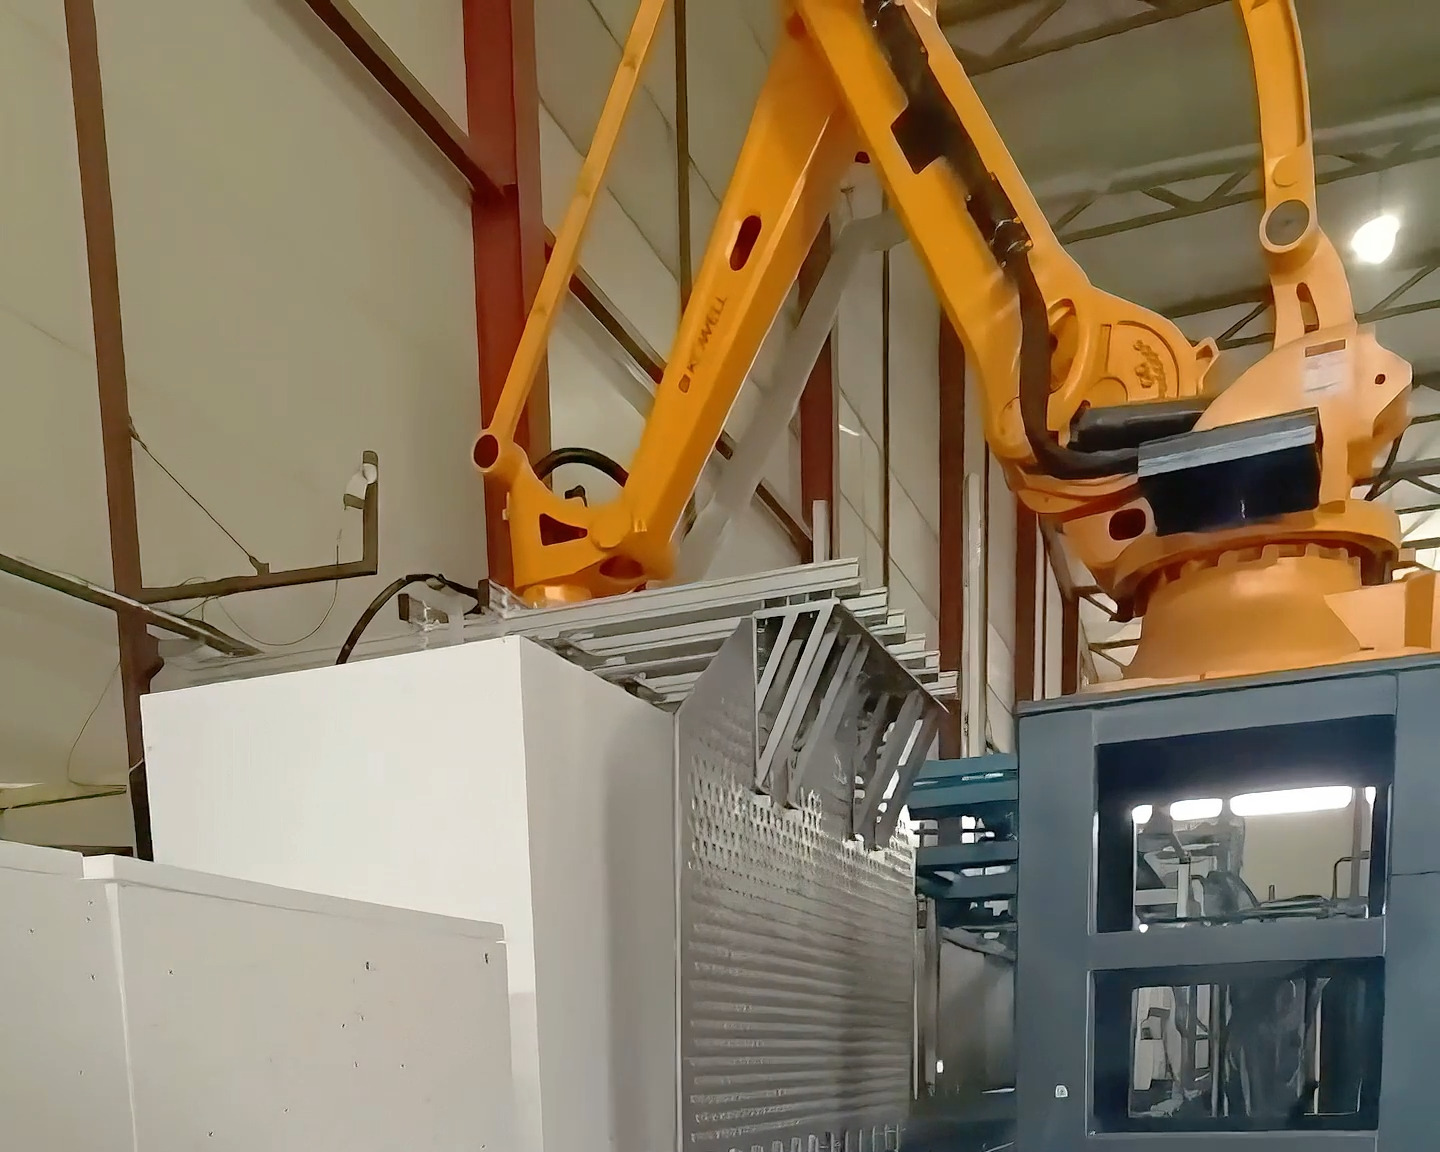
\includegraphics[width=0.44\textwidth]{figures/images/3DCloneEvroplast-real.jpg} &
  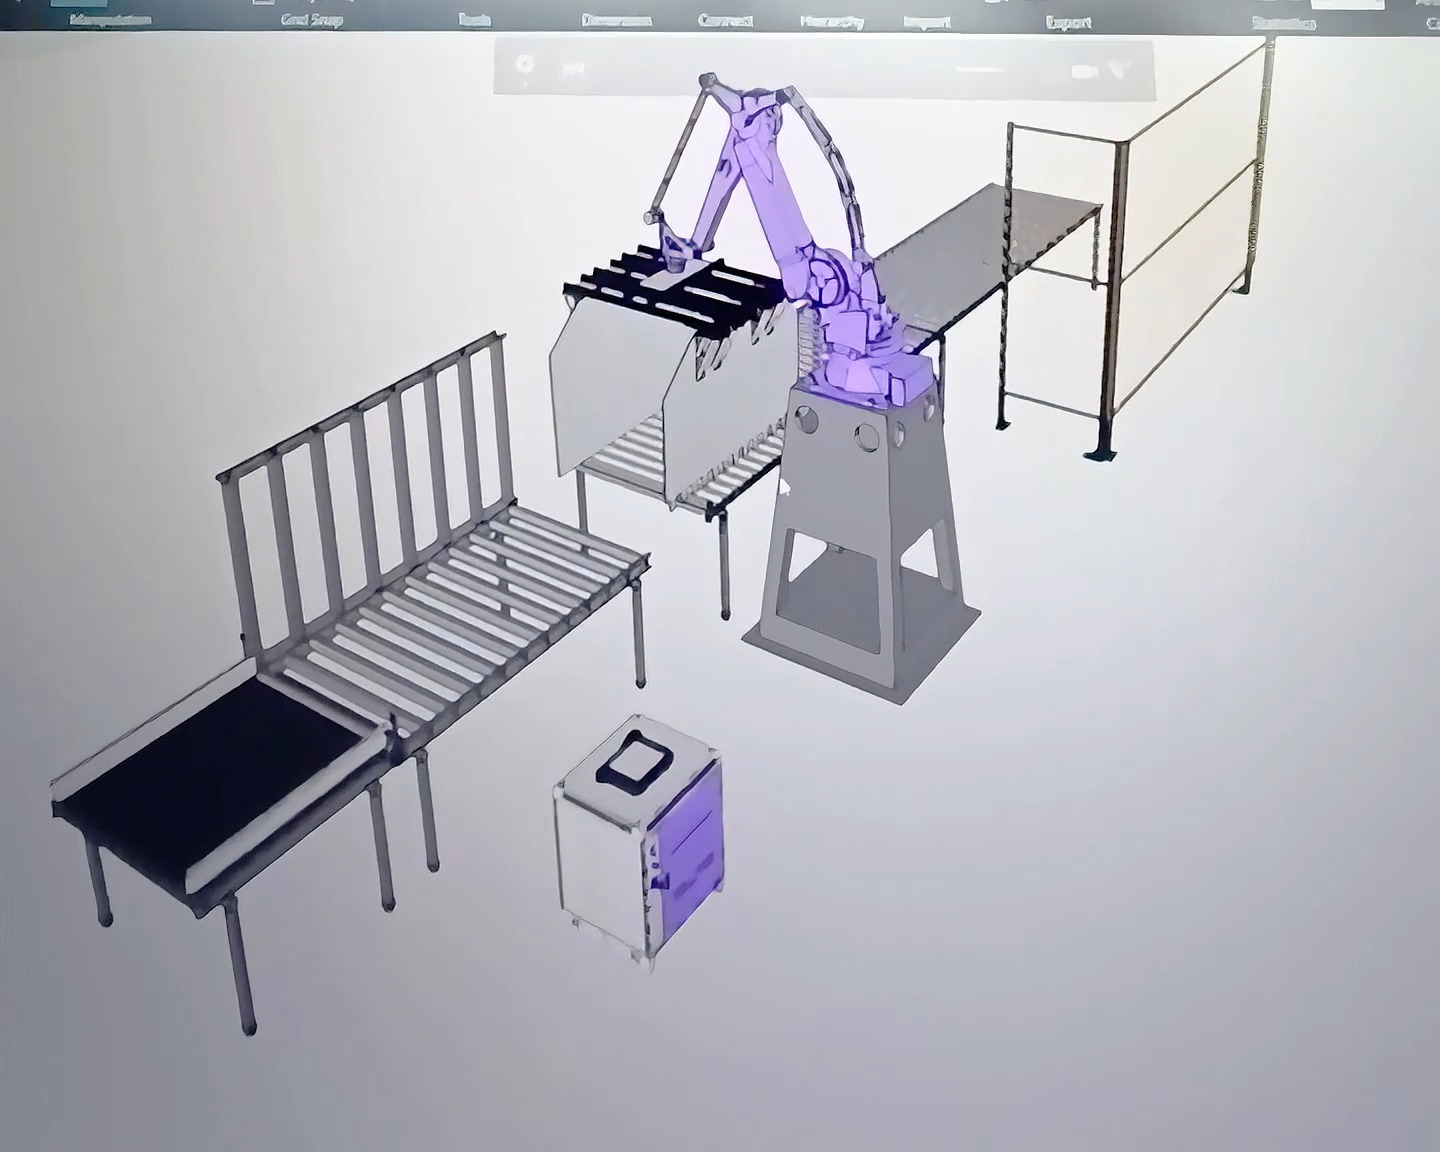
\includegraphics[width=0.44\textwidth]{figures/images/3DCloneEvroplast-double.jpg} \\
  а) реальный робот & б) цифровой двойник \\
\end{tabular}
\caption{Промышленный манипулятор и его цифровой двойник. Публикуется с разрешения ООО «Некстген Роботикс»}
\label{fig:digital_twin}
\end{figure}

\subsection{Выводы по разделу}

Таким образом, физическая симуляция в робототехнике решает качественно разные задачи --- от оффлайнового 
проектирования до обучения в реальном времени. Каждая задача предъявляет свои требования к физическому движку: 
SIL-тестирование требует детерминированности и работы в реальном времени, обучение с подкреплением --- 
максимальной производительности при запуске тысяч параллельных сред, цифровые двойники --- высокой точности и 
интеграции с внешними системами. Разрабатываемый физический движок должен удовлетворять всем перечисленным 
требованиям в рамках единой архитектуры.
